\باب{فوریئر تسلسل}
انجینئری مسائل میں دوری تفاعل عموماً پائے جاتے ہیں جن کو سادہ دوری تفاعل مثلاً \عددی{\sin} اور \عددی{\cos} کی روپ میں لکھنا مفید ثابت ہوتا ہے۔اسی عمل سے فوریئر تسلسل\حاشیہد{فرانسیسی ریاضی دان اور ماہر طبیعیات جین بپٹسٹ یوسف فوریئر [1768-1830]} ابھر کر سامنے آتی ہے جو سادہ تفرقی مساوات اور جزوی تفرقی مساوات کے حل میں کلیدی کردار ادا کرتی ہے۔

فوریئر تسلسل کا نظریہ پیچیدہ ہے جبکہ اس کا استعمال نہایت آسان  ہے۔چونکہ بہت سارے غیر استمراری تفاعل کا فوریئر تسلسل حاصل کرنا ممکن ہے جبکہ ان کا ٹیلر تسلسل نہیں پایا جاتا ہے لہٰذا فوریئر تسلسل کو ٹیلر تسلسل کی عالمگیر صورت تصور کیا جا سکتا ہے۔

اس باب میں فوریئر تسلسل سے وابستہ تصورات، حقائق اور تکنیکی تراکیب پر غور کیا جائے گا۔اس کے علاوہ ان کی استعمال پر غور کیا جائے گا۔اگلے باب میں جزوی تفرقی مساوات کی حل میں ان کا استعمال دکھایا جائے گا۔

اس باب کی آخری حصے میں فوریئر تکمل پر غور کیا جائے گا جنہیں اگلے باب میں جزوی تفرقی مساوات کی حل میں استعمال کیا جائے گا۔

\حصہ{دوری تفاعل، تکونیاتی تسلسل}
تفاعل \عددی{f(x)} اس صورت \اصطلاح{دوری}\فرہنگ{دوری}\حاشیہب{periodic}\فرہنگ{periodic} کہلاتا ہے کہ جب پورے حقیقی \عددی{x} پر \عددی{f(x)} معین ہو اور ایسا مثبت عدد \عددی{T} پایا جاتا ہو کہ تمام \عددی{x} پر درج ذیل درست ہو۔
\begin{align}\label{مساوات_فوریئر_دوری_تعریف_الف}
f(x+T)=f(x)\quad \quad \quad \text{\RL{تمام $x$ کے لئے}}
\end{align} 
عددی \عددی{T} کو \عددی{f(x)} کا \اصطلاح{دوری عرصہ}\فرہنگ{دوری عرصہ}\حاشیہب{period}\فرہنگ{period} کہتے\حاشیہد{تفاعل \عددی{f(x)} کا کم تر دوری عرصہ  \عددی{T (>0)}، اگر موجود ہو، \عددی{f(x)} کا اوّلی دوری عرصہ کہلاتا ہے۔مثلاً \عددی{\sin x} اور \عددی{\sin 2x} کا بالترتیب اوّلی دوری عرصہ \عددی{2\pi} اور \عددی{\pi} ہے جبکہ \عددی{f=\text{مستقل}} کا کوئی دوری عرصہ نہیں پایا جاتا ہے۔} ہیں۔\عددی{T} کے برابر  \عددی{f(x)} کے کسی بھی وقفے کا ترسیم دہراتے ہوئے ایسے تفاعل کا ترسیم حاصل کیا جاتا ہے (شکل \حوالہ{شکل_فوریئر_دوری_تفاعل})۔عملی استعمال میں عموماً  دوری اعمال اور تفاعل  پائے جاتے ہیں۔
\begin{figure}
\centering
\begin{tikzpicture}
\draw(-3,0)--(5,0)node[right]{$x$};
\draw(0,-1.2)--(0,1.2)node[left]{$f(x)$};
\draw[domain=-400:850,samples=100] plot ({\x/200},{0.5*sin(\x)-0.5/2*sin(2*\x)});
\draw(237/200,-0.6)--++(0,-0.3)coordinate[pos=0.75](kA);
\draw(237/200+360/200,-0.6)--++(0,-0.3)coordinate[pos=0.75](kB);
\draw[stealth-stealth] (kA)--(kB)node[pos=0.5,fill=white]{$T$};
\end{tikzpicture}
\caption{دوری تفاعل}
\label{شکل_فوریئر_دوری_تفاعل}
\end{figure} 

دوری تفاعل کی مثالیں \عددی{\sin x} اور \عددی{\cos x} ہیں۔اس کے علاوہ \عددی{f=c=\text{مستقل}} بھی دوری تفاعل کی تعریف (مساوات \حوالہ{مساوات_فوریئر_دوری_تعریف_الف} پر ہر مثبت \عددی{T} کے لئے) پورا اترنے کی بنا  دوری تفاعل ہے۔

مساوات \حوالہ{مساوات_فوریئر_دوری_تعریف_الف} سے ظاہر ہے کہ عدد صحیح \عددی{n} کی صورت میں درج ذیل ہو گا۔
\begin{align*}
f(x+nT)=f(x)\quad \quad \quad \text{\RL{تمام $x$ کے لئے}}
\end{align*}
یوں \عددی{2T}، \عددی{3T}، \عددی{4T}، \نقطے بھی تفاعل \عددی{f(x)} کے دوری عرصے ہیں۔مزید اگر تفاعل \عددی{f(x)} کا اور \عددی{g(x)} کا دوری عرصہ \عددی{T} ہو تب درج ذیل تفاعل
\begin{align*}
h(x)=af(x)+bg(x)\quad \quad \text{\RL{مستقل $a$، $b$}}
\end{align*}
 کا دوری عرصہ بھی \عددی{T} ہو گا جہاں \عددی{a} اور \عددی{b} مستقل ہیں۔

اس باب کی شروع میں ہم ایسے مختلف تفاعل جن کا دوری عرصہ \عددی{2\pi} ہو کو درج ذیل سادہ تفاعل کی  روپ میں ظاہر کرنا سیکھیں گے
\begin{align*}
1,\quad \cos x,\, \sin x,\quad \cos 2x,\, \sin 2x,\,\cdots, \quad \cos nx,\, \sin nx,\,\cdots
\end{align*}
جن کا دوری عرصہ \عددی{2\pi} ہے (شکل \حوالہ{شکل_فوریئر_سائن_کوسائن_یکساں_دوری_عرصہ})۔ہم دیکھیں گے کہ  ایسا کرتے ہوئے درج ذیل طرز کی تسلسل حاصل ہو گی
\begin{align}\label{مساوات_فوریئر_دوری_تعریف_ب}
a_0+a_1\cos x+b_1\sin x+a_2\cos 2x+b_2\sin 2x+\cdots
\end{align}
جہاں \عددی{a_0}، \عددی{a_1}، \عددی{a_2}،\نقطے، \عددی{b_1}،\عددی{b_2}،\نقطے حقیقی مستقل ہوں گے۔اس تسلسل کو \اصطلاح{تکونیاتی تسلسل}\فرہنگ{تسلسل!تکونیاتی}\حاشیہب{trigonometric series}\فرہنگ{series!trigonometric} کہتے ہیں جبکہ \عددی{a_n} اور \عددی{b_n} تسلسل کی \اصطلاح{عددی سر}\فرہنگ{عددی سر}\حاشیہب{coefficients}\فرہنگ{coefficients} کہلاتے ہیں۔چونکہ اس تسلسل کے ہر رکن کا دوری عرصہ \عددی{2\pi} ہے لہٰذا اگر یہ تسلسل مرکوز ہو تب یہ ایسا تفاعل ہو گا جس کا دوری عرصہ \عددی{2\pi} ہو گا۔
 
\begin{figure}
\centering
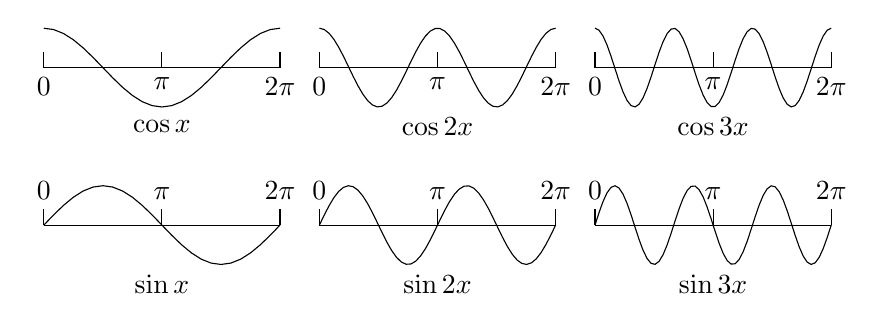
\begin{tikzpicture}
\pgfmathsetmacro{\amp}{0.5}
\pgfmathsetmacro{\pp}{120}
%
\draw(0,0)--(360/\pp,0);
\foreach \x/\l in {0/0,1.5/\pi,3/2\pi}{\draw(\x,0)node[below]{$\l$}--++(0,0.2);}
\draw[domain=0:360] plot ({\x/\pp},{\amp*cos(\x)});
\draw(1.5,-1.5*\amp)node{$\cos x$};
%
\begin{scope}[shift={(0,-4*\amp)}]
\draw(0,0)--(360/\pp,0);
\foreach \x/\l in {0/0,1.5/\pi,3/2\pi}{\draw(\x,0)--++(0,0.2)node[above]{$\l$};}
\draw[domain=0:360] plot ({\x/\pp},{\amp*sin(\x)});
\draw(1.5,-1.5*\amp)node{$\sin x$};
\end{scope}
%===========================
\begin{scope}[shift={(3.5,0)}]
\draw(0,0)--(360/\pp,0);
\foreach \x/\l in {0/0,1.5/\pi,3/2\pi}{\draw(\x,0)node[below]{$\l$}--++(0,0.2);}
\draw[domain=0:360,samples=50] plot ({\x/\pp},{\amp*cos(2*\x)});
\draw(1.5,-1.5*\amp)node{$\cos 2x$};
%
\begin{scope}[shift={(0,-4*\amp)}]
\draw(0,0)--(360/\pp,0);
\foreach \x/\l in {0/0,1.5/\pi,3/2\pi}{\draw(\x,0)--++(0,0.2)node[above]{$\l$};}
\draw[domain=0:360,samples=50] plot ({\x/\pp},{\amp*sin(2*\x)});
\draw(1.5,-1.5*\amp)node{$\sin 2x$};
\end{scope}
\end{scope}
%================================
\begin{scope}[shift={(7,0)}]
\draw(0,0)--(360/\pp,0);
\foreach \x/\l in {0/0,1.5/\pi,3/2\pi}{\draw(\x,0)node[below]{$\l$}--++(0,0.2);}
\draw[domain=0:360,samples=60] plot ({\x/\pp},{\amp*cos(3*\x)});
\draw(1.5,-1.5*\amp)node{$\cos 3x$};
%
\begin{scope}[shift={(0,-4*\amp)}]
\draw(0,0)--(360/\pp,0);
\foreach \x/\l in {0/0,1.5/\pi,3/2\pi}{\draw(\x,0)--++(0,0.2)node[above]{$\l$};}
\draw[domain=0:360,samples=60] plot ({\x/\pp},{\amp*sin(3*\x)});
\draw(1.5,-1.5*\amp)node{$\sin 3x$};
\end{scope}
\end{scope}
\end{tikzpicture}
\caption{سائن اور کوسائن تفاعل جن کا دوری عرصہ $2\pi$ ہے}
\label{شکل_فوریئر_سائن_کوسائن_یکساں_دوری_عرصہ}
\end{figure}

انجینئری میں واقع تفاعل پیچیدہ  ہوتے ہیں جنہیں سادہ دوری تفاعل کی روپ میں لکھنا مدد گار ثابت ہوتا ہے۔ہم دیکھیں گے کہ عملی استعمال، مثلاً ارتعاش، میں پائے جانے والا  تقریباً ہر دوری تفاعل \عددی{f(x)} جس کا دوری عرصہ \عددی{2\pi} ہو  کو فوریئر تسلسل کی روپ میں لکھنا ممکن ہو گا۔ہم مساوات \حوالہ{مساوات_فوریئر_دوری_تعریف_ب} کے عددی سر حاصل کرنے کے ایسے کلیات دریافت کریں گے جو \عددی{f(x)} پر منحصر ہوں گے اور جنہیں استعمال کرتے ہوئے حاصل تسلسل مرکوز ہو گا جس کا مجموعہ \عددی{f(x)} کے برابر ہو گا۔اس کے بعد ہم حاصل کلیات کو عمومی شکل دیتے ہوئے ان  کو کسی بھی دوری عرصہ کے تفاعل کے لئے قابل استعمال بنائیں گے۔ایسا کرنا نہایت آسان ثابت ہو گا۔

%============================
\حصہء{سوالات}

%===================
\ابتدا{سوال}\شناخت{سوال_فوریئر_کمتر_دوری_عرصہ_الف}\quad دیے گئے تفاعل کا کم تر دوری عرصہ دریافت کریں۔
\begin{align*}
\cos x,\, \sin x,\, \cos 2x,\, \sin 2x,\, \cos \pi x,\, \sin \pi x,\, \cos 2\pi x,\, \sin 2\pi x
\end{align*}
جوابات:\quad
$2\pi, 2\pi,\pi, \pi,2,2,1,1$

\انتہا{سوال}
%======================
\ابتدا{سوال}\quad اگر تفاعل \عددی{f(x)} کا دوری عرصہ \عددی{T} ہو تب ثابت کریں کہ \عددی{nT} جہاں \عددی{n=2,3,\cdots} ہے بھی اس تفاعل کا دوری عرصہ ہو گا۔
\انتہا{سوال}
%=====================
\ابتدا{سوال}\quad ثابت کریں کہ اگر تفاعل \عددی{f(x)} کا  اور تفاعل \عددی{g(x)} کا دوری عرصہ \عددی{T} ہو تب تفاعل \عددی{h(x)=af(x)+bg(x)} کا دوری عرصہ بھی \عددی{T} ہو گا، جہاں \عددی{a} اور \عددی{b} مستقل ہیں۔یوں دوری عرصہ \عددی{T} رکھنے والے تمام تفاعل سمتی فضا پیدا کرتے ہیں۔
\انتہا{سوال}
%=====================
\ابتدا{سوال}\quad ثابت کریں کہ تفاعل \عددی{f(x)=\text{مستقل}} ایسا دوری تفاعل ہے جس کا دوری عرصہ \عددی{T} کوئی بھی مثبت عدد ہو سکتا ہے۔
\انتہا{سوال}
%========================
\ابتدا{سوال}\quad ثابت کریں کہ  تفاعل \عددی{f(x)} کا دوری عرصہ \عددی{T} ہونے کی صورت میں \عددی{x} کے دوری تفاعل  \عددی{f(ax), a\ne 0} کا دوری عرصہ \عددی{\tfrac{T}{a}} ہو گا جبکہ \عددی{x} کے دوری  تفاعل \عددی{f(\tfrac{x}{b}), b\ne 0}  کا دوری عرصہ \عددی{bT} ہو گا۔ان نتائج کی تصدیق \عددی{f(x)=\cos x,\, a=b=2} کے لئے کریں۔ 
\انتہا{سوال}
%========================
سوال \حوالہ{سوال_فوریئر_ترسیم_کھینچیں_الف} تا سوال \حوالہ{سوال_فوریئر_ترسیم_کھینچیں_ب} میں دیے گئے تفاعل کا ترسیم کھینچیں۔

%===============
\ابتدا{سوال}\شناخت{سوال_فوریئر_ترسیم_کھینچیں_الف}\quad
$\sin x,\quad \sin x+\frac{1}{3}\sin 3x,\quad \sin x+\frac{1}{3}\sin 3x+\frac{1}{5}\sin 5x$

\انتہا{سوال}
%==========================
\ابتدا{سوال}\quad \عددی{f(x+2\pi)=f(x)} اور
\begin{align*}
f(x)=
\begin{cases}
-\frac{\pi}{4}& -\pi \le x \le 0\\
\phantom{-}\frac{\pi}{4}&\phantom{-}0\le x \le \pi
\end{cases}
\end{align*}
ہے۔سوال \حوالہ{سوال_فوریئر_ترسیم_کھینچیں_الف} کی ترسیم کے ساتھ موازنہ کریں۔
\انتہا{سوال}
%======================
\ابتدا{سوال}
\begin{align*}
\sin 2\pi x,\quad \sin 2\pi x+\frac{1}{3}\sin 6\pi x,\quad \sin 2\pi x+\frac{1}{3}\sin 6\pi x+\frac{1}{5}\sin 10\pi x
\end{align*}
\انتہا{سوال}
%========================
\ابتدا{سوال}
\begin{align*}
\sin x,\quad \sin x-\frac{1}{2}\sin 2x,\quad \sin x-\frac{1}{2}\sin 2x+\frac{1}{3}\sin 3x,\\
f(x)=\frac{x}{2}, \quad  -\pi \le x \le \pi, \quad f(x+2\pi)=f(x)
\end{align*}
\انتہا{سوال}
%========================
\ابتدا{سوال}
\begin{align*}
-\cos x,\quad -\cos x+\frac{1}{4}\cos 2x,\quad -\cos x+\frac{1}{4}\cos 2x-\frac{1}{9}\cos 3x,\\
f(x)=\frac{x^2}{4}-\frac{\pi^2}{12}, \quad  -\pi \le x \le \pi, \quad f(x+2\pi)=f(x)
\end{align*}
\انتہا{سوال}
%================================
\ابتدا{سوال}\quad 
$f(x)=x^2,\quad -\pi \le x \le \pi, \quad f(x+2\pi)=f(x)$
\انتہا{سوال}
%=======================
\ابتدا{سوال}\شناخت{سوال_فوریئر_ترسیم_کھینچیں_ب}\quad 
$f(x)=e^{\abs{x}},\quad -\pi \le x \le \pi, \quad f(x+2\pi)=f(x)$
\انتہا{سوال}
%=======================
